%   DOCUMENT CLASS  %%%%%%%%%%%%%%%%%%%%%%%%%%%%%%%%%%%%%%%%%%%%%%%%%%%%%%%%%%%
%
%   Use the `sfuthesis` class to format your thesis.
%
%   For more information about thesis formatting requirements, go to
%   http://www.lib.sfu.ca/help/publish/thesis or ask a thesis advisor at the
%   SFU Research Commons.


\documentclass{sfuthesis}



%   DOCUMENT METADATA  %%%%%%%%%%%%%%%%%%%%%%%%%%%%%%%%%%%%%%%%%%%%%%%%%%%%%%%%
%
%   Fill in the following information for the title page and declaration of
%   committee page. Please review the Declaration of Committee page
%   instructions on the library's thesis website before completing this page:
%   https://www.lib.sfu.ca/help/publish/thesis/format/declaration-committee

%   Choose the \faculty entry below from the following list:
%
%       - Faculty of Applied Sciences
%       - Faculty of Arts and Social Sciences
%       - Beedie School of Business
%       - Faculty of Communication, Art and Technology
%       - Faculty of Education
%       - Faculty of Environment
%       - Faculty of Health Sciences
%       - Faculty of Science

\title{Computational strategies for the nonlinear elastodynamics of skeletal muscle tissue}
\thesistype{Thesis}
\author{Javier Alejandro Almonacid Paredes}
\previousdegrees{%
    M.Sc., Simon Fraser University, 2020\\
    B.Sc., Universidad de Concepci\'{o}n, 2015}
\degree{Doctor of Philosophy}
\department{Department of Mathematics}
\faculty{Faculty of Science}
\copyrightyear{2025}
\semester{Spring 2025}


%   You may include up to six keywords or phrases. Keywords should be separated
%   with semicolons. No punctuation at the end.
\keywords{thesis template; Simon Fraser University; \LaTeX; time travel paradoxes}

\committee{
    \chair{TBD}{Professor \\ Department of Mathematics}
    \member{Nilima Nigam}{Supervisor \\ Professor \\ Department of Mathematics}
    \member{James Wakeling}{Committee Member (?)\\ Professor \\ Department of Biomedical Physiology and Kinesiology}
    \member{TBD}{Internal Examiner \\ Professor \\ Department of Mathematics}
    \member{TBD}{External Examiner \\ Professor \\ Department of Quantum Fields \\ Mars University}
}



%   PACKAGES %%%%%%%%%%%%%%%%%%%%%%%%%%%%%%%%%%%%%%%%%%%%%%%%%%%%%%%%%%%%%%%%%%
%
%   Add any packages you need for your thesis here.
%   You don't need to call the following packages, which are already called in
%   the sfuthesis class file:
%
%   - appendix
%   - etoolbox
%   - fontenc
%   - geometry
%   - lmodern
%   - nowidow
%   - setspace
%   - tocloft
%
%   If you call one of the above packages (or one of their dependencies) with
%   options, you may get a "Option clash" LaTeX error. If you get this error,
%   you can fix it by removing your copy of \usepackage and passing the options
%   you need by adding
%
%       \PassOptionsToPackage{<options>}{<package>}
%
%   before \documentclass{sfuthesis}.
%
%   The following packages are a few suggestions you might find useful.
%
%   (1) amsmath and amssymb are essential if you have math in your thesis;
%       they provide useful commands like ``blackboard bold'' symbols and
%       environments for aligning equations.
%   (2) amsthm includes allows you to easily change the style and numbering of
%       theorems. It also provides an environment for proofs.
%   (3) graphicx allows you to add images with \includegraphics{filename}.
%   (4) hyperref turns your citations and cross-references into clickable
%       links, and adds metadata to the compiled PDF.
%   (5) pdfpages lets you import pages of external PDFs using the command
%       \includepdf{filename}. You will need to do this if your research
%       requires an Ethics Statement.
%

\usepackage{amsmath}                            % (1)
\usepackage{amssymb}                            % (1)
\usepackage{amsthm}                             % (2)
\usepackage{graphicx}                           % (3)
\graphicspath{{figs/}}
\usepackage{epstopdf}
\usepackage[pdfborder={0 0 0}]{hyperref}        % (4)
% \usepackage{pdfpages}                         % (5)
% ...
% ...
% ...
% ... add your own packages here!

\usepackage{background}
\backgroundsetup{
  position=current page.north,
  angle=0,
  nodeanchor=north,
  vshift=-10mm,
  opacity=1,
  scale=1.5,
  contents=Submitted for revision on \today
}

\usepackage{circuitikz}
\usetikzlibrary{patterns,
                hobby,
                decorations.pathmorphing,
                shapes.geometric}

\usepackage{makecell}


%   OTHER CUSTOMIZATIONS %%%%%%%%%%%%%%%%%%%%%%%%%%%%%%%%%%%%%%%%%%%%%%%%%%%%%%
%
%   Add any packages you need for your thesis here. We've started you off with
%   a few suggestions.
%
%   (1) Use a single word space between sentences. If you disable this, you
%       will have to manually control spacing around abbreviations.
%   (2) Correct the capitalization of "Chapter" and "Section" if you use the
%       \autoref macro from the `hyperref` package.
%   (3) The LaTeX thesis template defaults to one-and-a-half line spacing. If
%       your supervisor prefers double-spacing, you can redefine the
%       \defaultspacing command.
%

\frenchspacing                                    % (1)
\renewcommand*{\chapterautorefname}{Chapter}      % (2)
\renewcommand*{\sectionautorefname}{Section}      % (2)
\renewcommand*{\subsectionautorefname}{Section}   % (2)
% \renewcommand{\defaultspacing}{\doublespacing}  % (3)
% ...
% ...
% ...
% ... add your own customizations here!

\usepackage{bm,bbm}
\usepackage{empheq}

%-----------------------------------------------
% Eliminate ugly boxes around references.
\usepackage{xcolor}
\hypersetup{
    colorlinks,
    linkcolor={red!50!black},
    citecolor={blue!50!black},
    urlcolor={blue!80!black}
}
%------------------------------------------------

\numberwithin{equation}{chapter}
\numberwithin{figure}{chapter}
\numberwithin{table}{chapter}


\newtheorem{objective}{Objective}
\renewcommand*{\theobjective}{\Alph{objective}}
\newtheorem{theorem}{Theorem}[chapter]
\newtheorem{remark}[theorem]{Remark}

\theoremstyle{definition}
\newtheorem{definition}{Definition}[chapter]
\newtheorem{lemma}[definition]{Lemma}
\newtheorem{example}[definition]{Example}

%%%%%%%%%%%%%%%%%%%%%%%%%%%%%%%%%%%%%%%%%%%%%%%%%%%
%
%  DEFINITIONS 
%
%%%%%%%%%%%%%%%%%%%%%%%%%%%%%%%%%%%%%%%%%%%%%%%%%%%

\def\*#1{{\mathbf{#1}}} % bold letters!
\newcommand{\pder}[2]{\dfrac{\partial #1}{\partial #2}}
\newcommand{\Dder}[2]{\dfrac{\mathrm{D} #1}{\mathrm{D} #2}}
\newcommand{\der}[2]{\dfrac{\mathrm{d} #1}{\mathrm{d} #2}}
\newcommand{\dder}[2]{\dfrac{\mathrm{d} #1}{\mathrm{d} #2}}
\newcommand{\divs}[1]{{\mathrm{div} \, #1}}
\newcommand{\Divs}[1]{{\mathrm{Div} \, #1}}
\newcommand{\divt}[1]{{\bm{\mathrm{div}} \, #1}}
\newcommand{\Divt}[1]{{\bm{\mathrm{Div}} \, #1}}

\newcommand{\depsilon}{\dot{\varepsilon}}
\newcommand{\R}{\mathbb{R}}
\newcommand{\B}{\mathcal{B}}
\newcommand{\F}{\mathcal{F}}
\newcommand{\I}{{\bar{I}}}
\newcommand{\FF}{{\bm{\mathcal{F}}}}
\newcommand{\C}{\mathbb{C}}
\newcommand{\T}{\top}
\renewcommand{\c}{\mathbbm{c}}
\renewcommand{\P}{\mathbb{P}}
\newcommand{\p}{\mathbbm{p}}
\newcommand{\vphi}{\varphi}
\newcommand{\matlab}{MATLAB\textsuperscript{\textcopyright} }

\def\bsigma{{\bm{\sigma}}}
\def\btau{{\bm{\tau}}}
\def\bchi{{\bm{\chi}}}
\def\bxi{{\bm{\xi}}}
\def\bphi{{\bm{\varphi}}}

\newcommand{\javicomment}[1]{\noindent {\color{red}\textbf{Comment by Javi: #1}}}

%%%%%%%%%%%%%%%%%%%%%%%%%%%%%%%%%%%%%%%%%%%%%%%%%%%
%
% END OF DEFINITIONS
%
%%%%%%%%%%%%%%%%%%%%%%%%%%%%%%%%%%%%%%%%%%%%%%%%%%%



%   FRONTMATTER  %%%%%%%%%%%%%%%%%%%%%%%%%%%%%%%%%%%%%%%%%%%%%%%%%%%%%%%%%%%%%%
%
%   Title page, committee page, abstract, dedication, acknowledgements, table
%   of contents, etc.
%
%   If your research requires an Ethics Statement, download the pdf from
%   https://www.lib.sfu.ca/help/publish/thesis/regulations#ethics-statement
%   to your thesis folder, then uncomment the appropriate lines below.

\begin{document}

\frontmatter
\maketitle{}
\makecommittee{}

%\addtoToC{Ethics Statement}%
%\includepdf[pagecommand={\thispagestyle{plain}}]{ethics_statement_piii.pdf}%
%\clearpage

\begin{abstract}
    %Skeletal muscle is a highly complex biological tissue capable of generating work and power for different tasks, such as postural control, locomotion, stabilization of bones and joints, and heat generation. Its mechanics involve several length scales, from cellular units in micrometres to the size of, for example, the sartorius muscle in larger mammals (in the scale of metres). Despite this intricacy, computational models of skeletal muscle typically neglect important features of whole muscles, such as size, shape, architecture, and mass, leading to models that are static or quasi-static. Perhaps surprisingly, many times this simplification is valid and incredibly helpful in predicting muscle function. However, in scenarios such as faster dynamics or whole-muscle dynamics, these often neglected characteristics have a heavy influence on the biomechanical output of computational models. The latter leads to fully dynamic models which are challenging to solve, making this a rather unexplored area in computational biomechanics.

    %In this thesis, we study the nonlinear elastodynamics of skeletal muscle tissue. The first part of this dissertation pertains to one-dimensional models. First, we study the inertial effects in a multi-body model of the muscle-tendon unit using experimentally obtained data. Then, we study the lack of stability in these multi-body models (a non-physical phenomenon) and propose a new continuum model that provides stability throughout the range of motion of a muscle. Next, as a preamble for the next part, we study time discretization options for Neo-Hookean deformation in the presence of a highly stiff material. The second part of this work corresponds to three-dimensional models. Here, we begin with a a new Lagrangian framework for a 3D model of skeletal muscle tissue which simplifies a previously-developed Eulerian model. Moreover, we introduce a new fully implicit time discretization. Then, we introduce Flexodeal, a new finite-element tool for studying musculoskeletal dynamics, completely open source and available to the public. Finally, using this newly developed software, we study gearing in muscle tissues. We show that Flexodeal not only provides results that are in line with literature findings but also provides a framework to study this phenomenon in a variety of muscle architectures and activation levels.
\end{abstract}


\begin{dedication}
This is an optional page. Use your choice of paragraph style for text on this page.
\end{dedication}


\begin{acknowledgements}
This is an optional page. Use your choice of paragraph style for text on this page.
\end{acknowledgements}

\addtoToC{Table of Contents}%
\hypersetup{linkbordercolor=black,hidelinks}
\tableofcontents%
\clearpage

%   This is an optional page. Remove the following lines if you don't have any tables.
\addtoToC{List of Tables}%
\listoftables%
\clearpage

%   This is an optional page. Remove the following lines if you don't have any figures.
\addtoToC{List of Figures}%
\listoffigures%
\clearpage





%   MAIN MATTER  %%%%%%%%%%%%%%%%%%%%%%%%%%%%%%%%%%%%%%%%%%%%%%%%%%%%%%%%%%%%%%
%
%   Start writing your thesis --- or start \include ing chapters --- here.
%

\mainmatter%

\chapter{Introduction}

Start writing or pasting in your text here. By default, only works cited in the text will be added to the bibliography~\cite{HolzapfelBook}.

\section{Physiology of skeletal muscle}

\section{State of the art in muscle modelling}

\section{Continuum mechanics of deformable solids}

This might be a long section, maybe could be a chapter at the beginning of part 2? Should include some comments on generic deformation $\rho_0 \*u_{tt} = \Divt{\*P} + \*f$ and reduction to 1D if this is left as a section in the Introduction.

\part{One-dimensional elastodynamics}

\chapter{Inertial effects in a multi-body mass-spring model of the muscle-tendon unit}

%Work with Evan on mass enhanced muscle models. We need to discuss what would be appropriate to show here, besides the model and the numerical strategy (dynamic/mass effects? Focus on one cycle? Effects of different muscles and activities?).
%Github repository: mass-enhanced-muscle-models.

%\medskip

%Things that are not in Evan's thesis:
%\begin{enumerate}
%    \item tendon dynamics
%    \item what happens as the number of masses increases (homogenization study)
%\end{enumerate}

%Understanding the elastodynamics of skeletal muscle requires us to have an idea on the expected behaviour of muscle models. As a first approach to this task, we consider one-dimensional actuators. These are models that are well-established in the literature and that are part of major biomechanics software, such as OpenSim and FEBio [REFS]. Despite their apparent simplicity, however, these models are typically made of one or more highly-nonlinear ODEs whose stiff character cannot be overlooked.

%\hrulefill

In this chapter, we study the inertial effects due to added mass in a particular set of forward dynamics simulations of muscle-tendon units (MTUs). More precisely, using locomotion data collected in studies by Chen \cite{EvanThesis} and Dick et al. \cite{Dick2016}, we compare the predictions of a multibody mass-spring model of the MTU against those of a simpler model widely used in biomechanical simulations. In addition, we investigate the influence of the input data in the numerical aspects of the problem. We show that they are not only are influenced by the stiffness of the system, but also by the muscle in consideration and the task is asked to perform.

First, we mathematically describe the ordinary differential equations (ODEs) and the different concepts behind MTU models. Next, we describe the data and parameters in use for this study. Then, we describe the computational implementation of the different solvers required to perform these simulations. Here, we aim to compute lengths and velocities for muscle and tendon, as well as muscle force. Finally, we present a series of tests which show that both models (with and without added mass) show different dynamics, reiterating the importance of considering mass in muscle models for certain experimental scenarios.

\section{Background}

One-dimensional models of skeletal muscle are effective in capturing the overall dynamics of skeletal muscle. Their relative simplicity allows physiologists to perform cheap forward dynamics simulations on a range of subjects, muscles, and tasks.

Consider, for instance, the protocol developed by Chen \cite{EvanThesis} to record data from a human subject during locomotion tasks. Here, 24 LED motion-capture markers are secured to the skin over the pelvis and lower extremities of each participant to capture kinematic and kinetic data. Furthermore, bipolar Ag/AgCl surface electromyography (EMG) electrodes are positioned over the bellies of 10 different muscles to capture EMG data. After this setup is complete, subjects asked to perform 4 different tasks (walking and running on a treadmill, hopping, and sit-to-stand from a chair) with appropriate breaks in between. Data is recorded for about 30 seconds per task and each task is repeated twice. This means that if data is collected for 20 subjects, up to $20 \times 10 \times 8 = 1600$ different simulations could be performed. Thus, accurate and efficient models and numerical algorithms are required to analyze the data in a feasible timeframe.

%In this project, we implement a set of MATLAB routines for a multi-body model of the muscle-tendon unit (MTU) developed by Chen in \cite{EvanThesis}, which has its origins on the work by G\"{u}nther et al. \cite{Gunther2012}, Ross \& Wakeling \cite{RossWakeling2016Multibody}, and Ross et al. \cite{Ross2018}. Moreover, we study the inertial (mass) effects in a particular subset of forward dynamics simulations using previously collected data \cite{EvanThesis,Dick2016}. These effects are typically neglected in the literature (e.g. in the popular biomechanics software OpenSim \cite{Delp2007OpenSim}), but several studies have consistently shown that there are certain scenarios where inertia is not negligible \cite{EvanThesis,RossWakeling2016Multibody}. First, we mathematically describe the ordinary differential equations (ODEs) describing these MTU models. Next, we describe the data and parameters in use for this study. Then, we describe the computational implementation of the solvers required for this study, which will compute important quantities, such as lengths and velocities for muscle and tendon, as well of muscle force. Finally, we describe the inertial effects observed in the simulations and compare these to the output of a typical model that does not take into account the mass of the muscle.

%Using the data collected in \cite{EvanThesis}, we consider two subjects\footnote{One subject performed walking and running tasks, while a different one performed the cycling task. Given that morphological differences are not considered in this study, we will treat these two subjects as a single one.} and select a set of three muscles: medial gastrocnemius (MG), vastus medialis (VM), and semitendinosus (ST); and a set of three tasks: walking, cycling, and running. 

\section{Mathematical models}

\begin{figure}
    \centering
    \includegraphics[width=0.9\textwidth]{mtu_sketch.jpeg}
    \caption{Sketch of an MTU (nicer version to come).}
    \label{fig:mtu_sketch}
\end{figure}

Let us develop a mathematical model of a dynamically contracting one-dimensional muscle tendon unit, such as the one depicted in Figure \ref{fig:mtu_sketch}. Denote by $L_M = L_M(t)$ and $L_T= L_T(t)$ the muscle and tendon lengths, respectively, at time $t \geq 0$. Moreover, denote by $L = L(t)$ the total length of the MTU which satisfies $L_M(t) + L_T(t) = L(t)$ for any time $t \geq 0$.

\subsection{Main concepts}

We define the \textit{muscle stretch} $\lambda_M$, the \textit{muscle strain} $\varepsilon_M$, and the \textit{muscle strain rate} $\depsilon_M$ as
\begin{equation} \label{eq:def_stretch_strain_rate_muscle}
    \lambda_M := \dfrac{L_M}{l_{mus}^{opt}}, \qquad \varepsilon_M := \lambda_M - 1, \qquad \depsilon_M = \dfrac{1}{\depsilon_0} \dder{\lambda_M}{t} = \dfrac{1}{l_{mus}^{opt} \, \depsilon_0} \dder{L_M}{t},
\end{equation}
where $l_{mus}^{opt}$ is the \textit{optimal muscle length} and $\depsilon_0$ is the maximum unloaded shortening strain rate. Similarly, we can define the \textit{tendon stretch} $\lambda_T$ and \textit{tendon strain} $\varepsilon_T$ as
\begin{equation}
    \lambda_T := \dfrac{L_T}{l^{opt}_{ten}}, \qquad \varepsilon_T := \lambda_T - 1.
\end{equation} 
The \textit{optimal tendon length} $l_{ten}^{opt}$ can be computed from the \textit{optimal MTU length} $l_{MTU}^{ten}$ as  $l_{ten}^{opt} = l_{MTU}^{opt} - l_{mus}^{opt}$. For now, the reader can consider these quantities as given, however, they will be discussed more in detail in Section \ref{sec:optimal_muscle_length}.



\subsection{Hill's muscle model}

In a simple model, such as the one shown in Figure \ref{fig:muscle_models_1D}A, muscle can be thought as a one-dimensional spring containing a contractile element (CE) and a parallel elastic element (PEE). The first one is related to the force produced by actin-myosin interactions during activation, whereas the latter is related to passive components of the muscle fibre (such as titin), which act to prevent overstretching of the sarcomeres that form the muscle fibre. The muscle force $F_M$ in this case is given by Hill's equation \cite{Zajac1989},
\begin{equation} \label{eq:Hill_force}
    F_{Hill}(\lambda_M, \depsilon_M) = F_0 \Big\{ a(t) \widehat{F}_A(\lambda_M) \widehat{F}_V(\depsilon_M) + \widehat{F}_P(\lambda_M) \Big\}.
\end{equation}
In this expression, known as the standard \textit{Hill's muscle model}:
\begin{enumerate}
    \item The maximum isometric force, $F_0$, is the maximum force that a muscle can produce during an isometric contraction (that is, a \textit{fixed}-length contraction). This force is achieved when the length of the muscle $L_M$ is exactly the optimal muscle length $l_{mus}^{opt}$. Therefore, it can be computed as:
    \begin{equation}
        F_0 = \sigma_0 \cdot PCSA_0 = \sigma_0 \cdot \dfrac{V_{0,mus}}{l_{mus}^{opt}},
    \end{equation}
    where $\sigma_0$ is the maximum isometric stress of muscle tissue, $PCSA_0$ is the optimal physiological cross-sectional area (PCSA), and $V_{0,mus}$ is the muscle volume.
    \item The time-dependent activation function, $a = a(t)$, characterizes the influx of $\mathrm{Ca}_2^+$ ions that trigger the formation of cross-bridges between actins and myosins within sarcomeres. This function can be computed given an excitation $u(t)$ using Zajac's equation \cite{Zajac1989}:
    \begin{equation} \label{eq:zajac}
        \dfrac{da}{dt} + \dfrac{a(t)}{\tau_{act}} \left( \beta + (1-\beta)u(t) \right) = \dfrac{u(t)}{\tau_{act}}.
    \end{equation}
    \item The functions $\widehat{F}_A = \widehat{F}_A(\lambda_M)$ and $\widehat{F}_V = \widehat{F}_V(\depsilon)$ are known respectively as the active \textit{force-length} (FL) and \textit{force-velocity} (FV) relationships. They are related to the CE of the model and describe the force produced due to actin-myosin interactions during activation. These are normalized functions, meaning that $\widehat{F}_A(1) = 1$ and $\widehat{F}_V(0) = 1$.
    \item The function $\widehat{F}_P = \widehat{F}_P(\lambda_M)$ is known as the passive FL relationship. It is related to the PEE and describes the force produced by passive components of the muscle fibre (such as titin), which act to prevent overstretching of the sarcomeres.
\end{enumerate} 

\begin{figure}
    \centering
    \begin{tikzpicture}[square/.style={regular polygon,regular polygon sides=4}]
        \node[inner sep=0pt] at (0,0)
            {\hspace{-3.5em}\includegraphics[width=1.18\textwidth]{force-curves-1D.png}};
        \node at (1.8,-1) [square,draw] {\large \phantom{A}};
        \draw[->] (2.2, -1) -- (3.8,-0.8);
    \end{tikzpicture}
    \caption{Force-relationships in use.}
    \label{fig:force_curves_1D}
\end{figure}

The force relationships $\widehat{F}_A$, $\widehat{F}_V$, and $\widehat{F}_P$ are typically fit from experimental data obtained through tensile experiments, and therefore do not have a standard expression. For this particular set of experiments, we use least-squares fits of the B\'{e}zier curves used by Ross et al. \cite{RossWakeling2016Multibody}. This allows us to evaluate the force directly given a stretch $\lambda_M$ without the need for solving a nonlinear equation, as is the case for B\'{e}zier curves (albeit with a minor loss of accuracy since the B\'{e}zier curves are already fit from experimental data). 
We portray these curves in Figure \ref{fig:force_curves_1D} and give their exact definitions in Appendix \ref{app:force_relationships}.

\begin{figure}
    \centering
    \begin{tikzpicture}
        \centering
        \node at (-2.8,1) {\huge \textbf{A}};
        \node[inner sep=0pt] at (0,0)
            {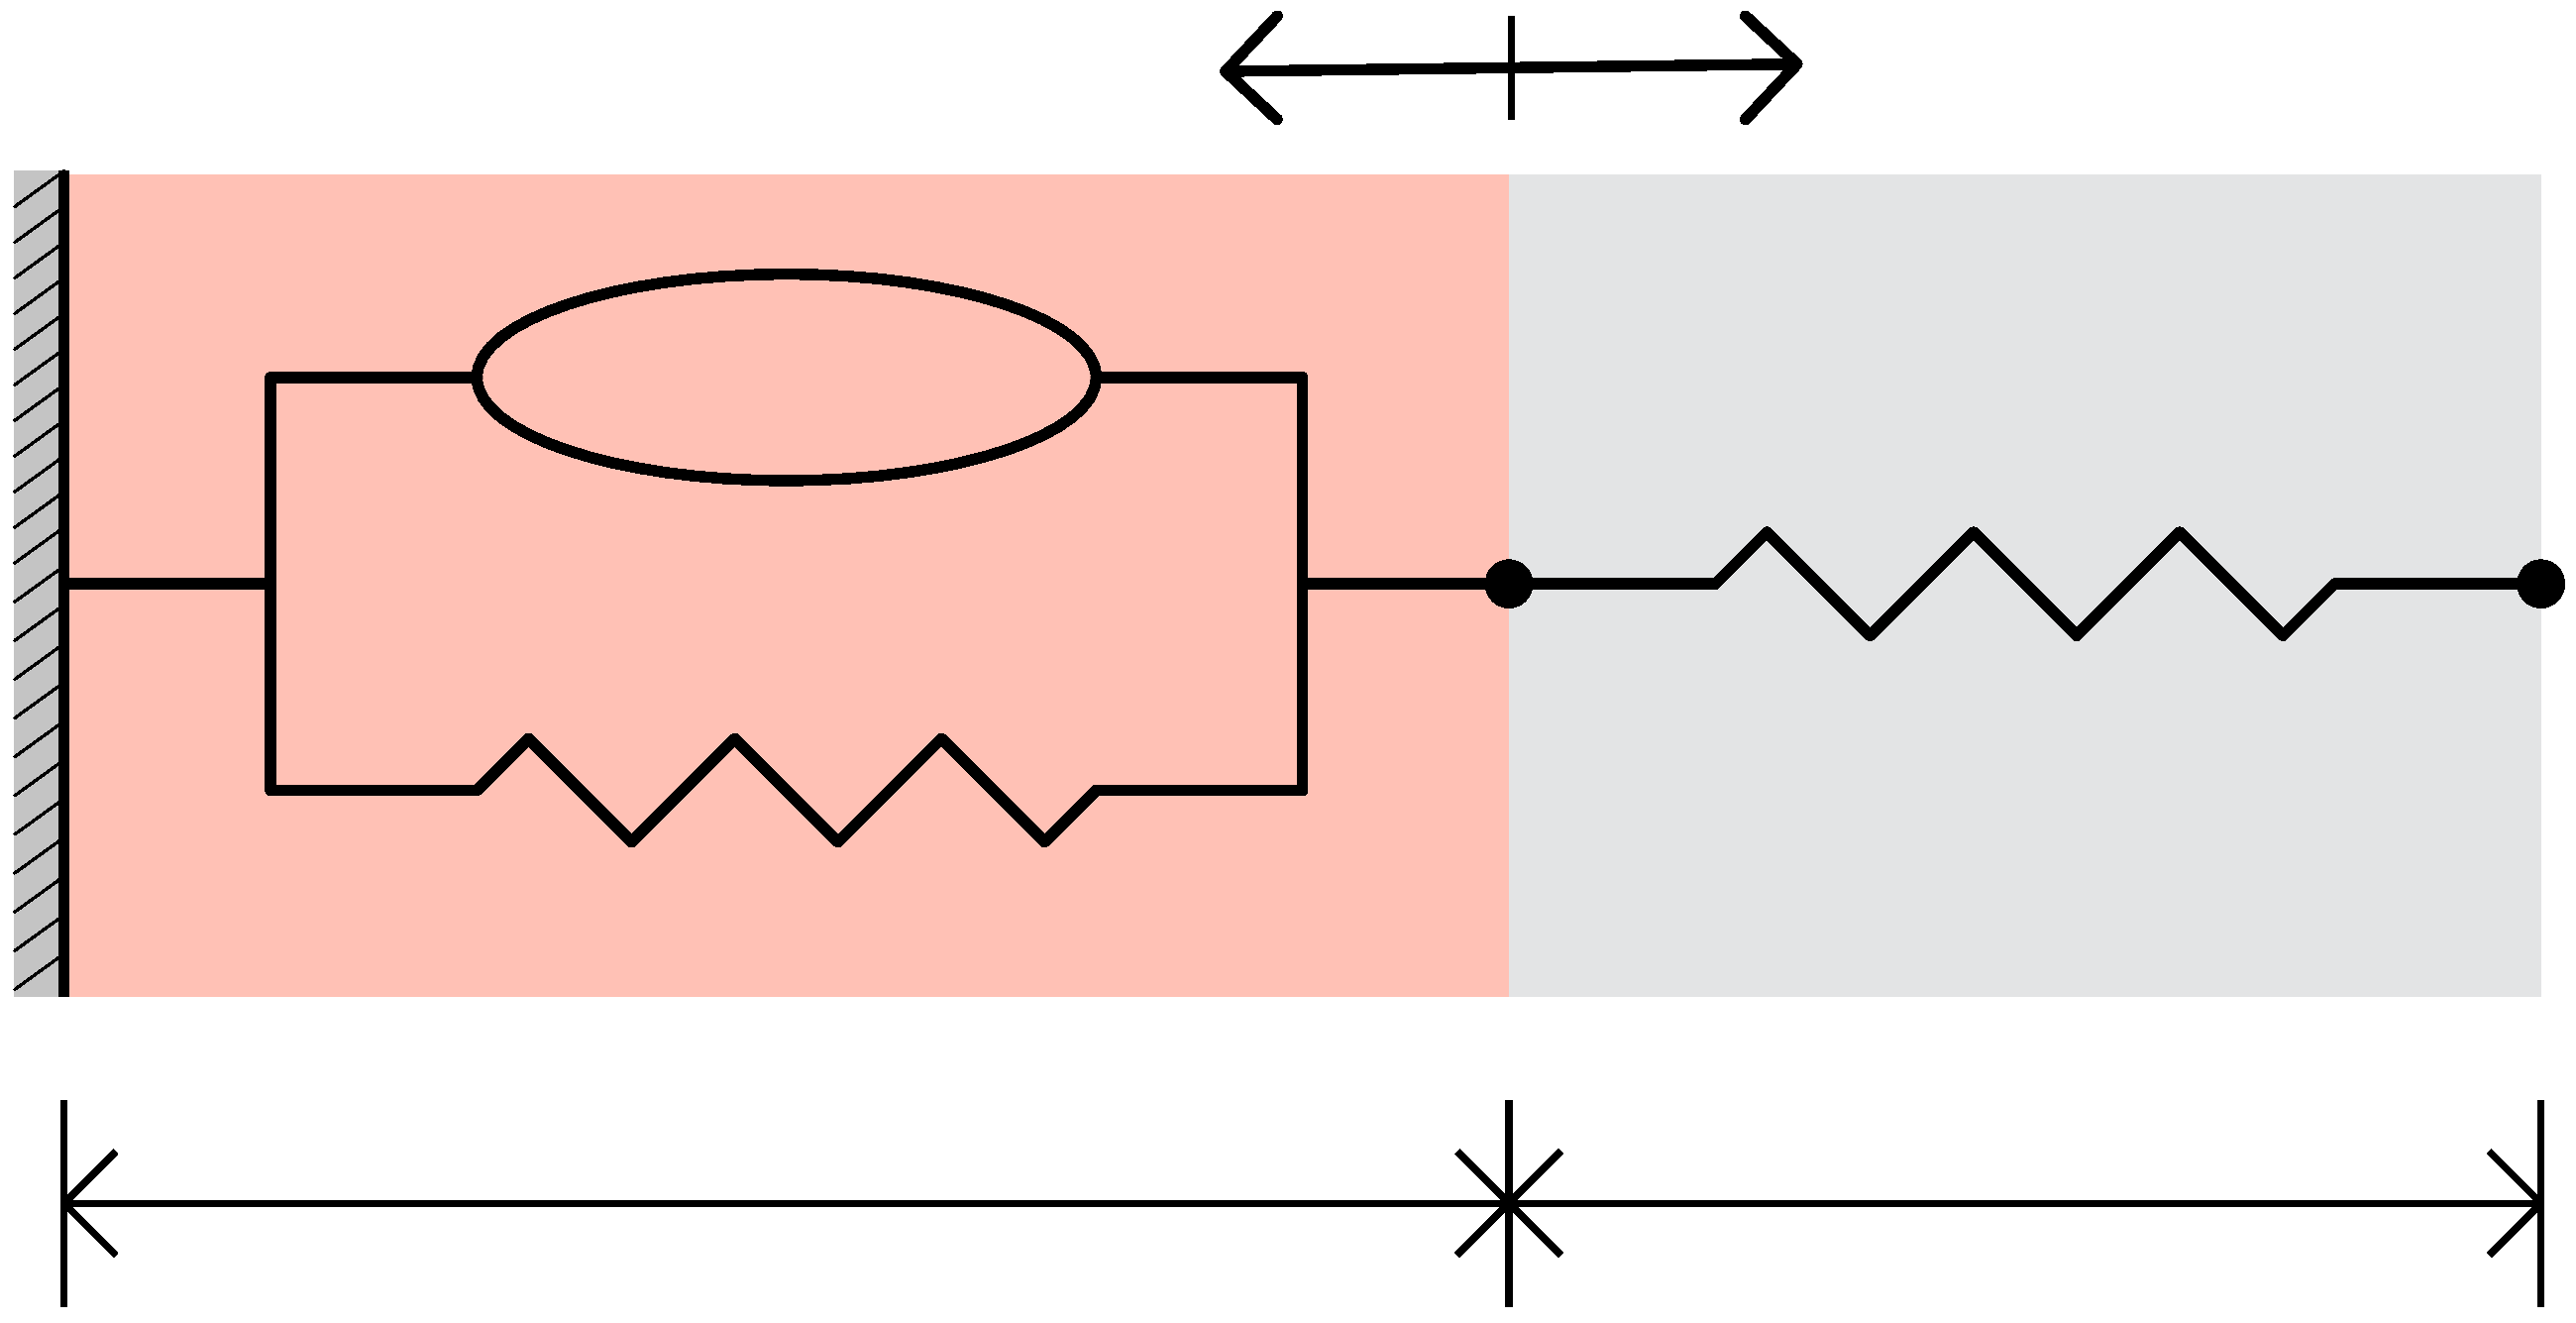
\includegraphics[width=0.3\textwidth]{hill-massless.eps}};
        \node at (-0.92,0.5) {\footnotesize CE};
        \node at (-0.92, -0.47) {\footnotesize PEE};
        \node at (1.33,-0.2) {SEE};
        \node at (-0.92, -1.25) {\footnotesize $L_M$};
        \node at (1.33, -1.25) {\footnotesize $L_T$};
        \node at (0.1, 1.45) {\footnotesize $\vec{F}_M$};
        \node at (0.7, 1.45) {\footnotesize $\vec{F}_T$};
    \end{tikzpicture}
    \hspace{0.5em}
    \begin{tikzpicture}
        \centering
        \node at (-4.5,1) {\huge \textbf{B}};
        \node[inner sep=0pt] at (0,0)
            {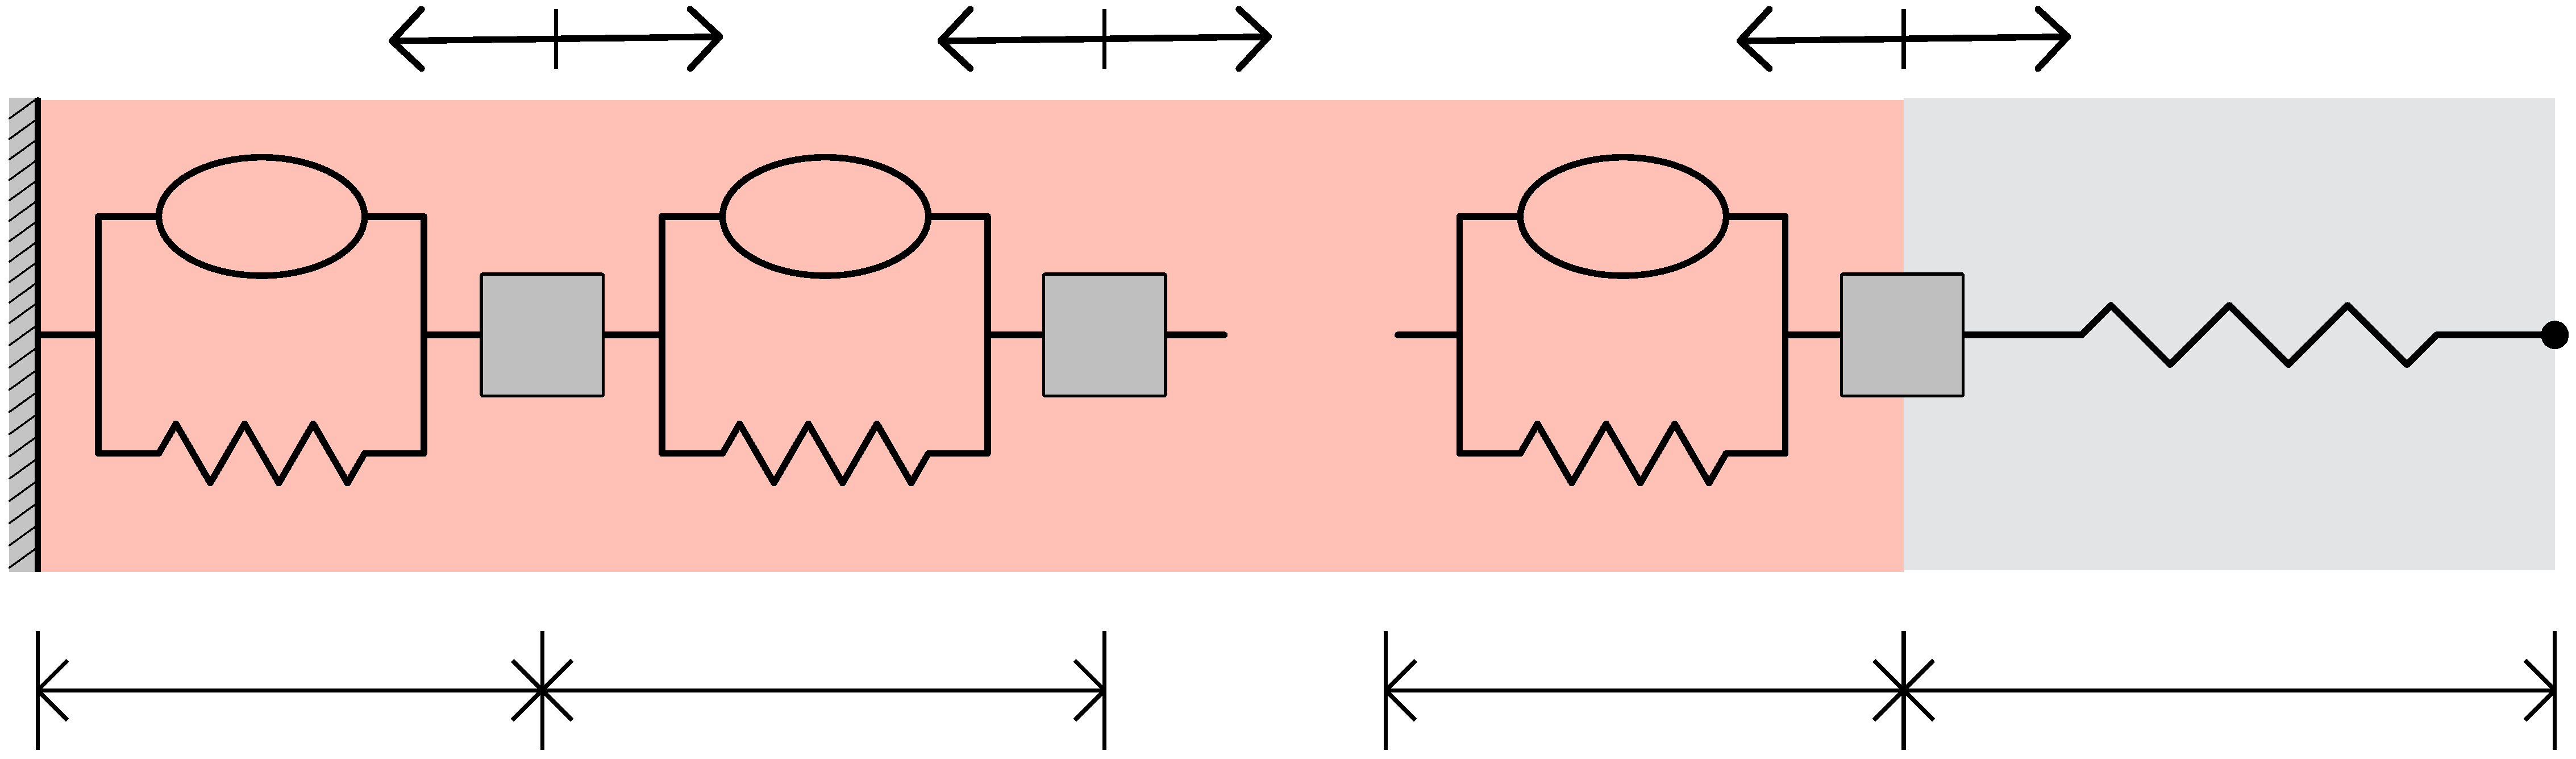
\includegraphics[width=0.525\textwidth]{hill-mass-enhanced.eps}};
        \node at (-2.31, 0.1) {\tiny $m_1$};
        \node at (-0.56, 0.1) {\tiny $m_2$};
        \node at (1.94, 0.1) {\tiny $m_{\hspace{-0.15em}N}$};
        \node at (-3.2, 0.5) {\tiny CE$_1$};
        \node at (-3.2, -0.5) {\tiny PEE$_1$};
        \node at (-3.2, -1.26) {\footnotesize $l_1$};
        \node at (-1.45, 0.5) {\tiny CE$_2$};
        \node at (-1.45, -0.5) {\tiny PEE$_2$};
        \node at (-1.45, -1.26) {\footnotesize $l_2$};
        \node at (1.08, 0.5) {\tiny CE$_{\hspace{-0.15em}N}$};
        \node at (1.08, -0.5) {\tiny PEE$_{\hspace{-0.15em}N}$};
        \node at (1.08, -1.26) {\footnotesize $l_N$};
        \node at (3.05, -0.2) {\tiny SEE};
        \node at (3.05, -1.26) {\footnotesize $L_T$};
        \node at (-2.6, 1.45) {\footnotesize $\vec{F}_1$};
        \node at (-2.0, 1.45) {\footnotesize $\vec{F}_2$};
        \node at (-0.9, 1.45) {\footnotesize $\vec{F}_2$};
        \node at (-0.3, 1.45) {\footnotesize $\vec{F}_3$};
        \node at (1.65, 1.45) {\footnotesize $\vec{F}_N$};
        \node at (2.25, 1.45) {\footnotesize $\vec{F}_T$};
        \node at (0.1,0.14) {\footnotesize $\dots$};
        \node at (-0.1,-1.0) {\footnotesize $\dots$};
    \end{tikzpicture}
    \caption{(A) A simple Hill-type model of the MTU (muscle region in pink, tendon region in grey) using massless springs. Depicted here are the (active) contractile element (CE), the passive elastic element (PEE), and the series elastic element (SEE) representing the tendon. (B) A multi-body model of the MTU that does not neglect the mass of the muscle, which is equally distributed throughout the muscle segment.}
    \label{fig:muscle_models_1D}
\end{figure}

%\begin{circuitikz}
    %ground
    %\pattern[pattern=north east lines] (0,0) rectangle (7,.25);
    %\draw[thick] (0,.25) -- (7,.25);
    
    %\draw (3,.25) to[spring, l=$k$] (3,2);
    %\draw (4,.25) to[damper, l_=$b$] (4,2);
    %\draw[fill=gray!40] (2.5,2) rectangle (4.5,3);
    %\node at (3.5,2.5) {$m$};
    
    %\draw[thick, ->] (3.5,4) -- (3.5,3);
    %\node at (3.75,3.75) {$F$};   
%\end{circuitikz}

%\begin{circuitikz}
    
    %\pattern[pattern=north east lines] (0,0) rectangle (0.2, 2);
    %\draw[thick] (0.2, 0) -- (0.2, 2);
    %\draw (0.2, 1) -- (0.8, 1);
    %\draw (0.8, 1) -- (0.8, 1.5) -- (1.3, 1.5);
    %\draw (1.9, 1.5) ellipse (6mm and 3mm);
    %\draw (2.5, 1.5) -- (3.0, 1.5);
    %\draw (0.8, 1) -- (0.8, 0.5) -- (1.0, 0.5);
    %\draw (1.0, 0.5) to[R] ++(1.8, 0) -- (3.0, 0.5);
    %\draw (3.0, 0.5) -- (3.0, 1.5);
    %\draw (3.0, 1.0) -- (3.6, 1.0);

%\end{circuitikz}

\subsection{Massless and mass-enhanced models of the MTU}

For the model in Figure \ref{fig:muscle_models_1D}A, the muscle force $F_M \equiv F_{Hill}$ is balanced by the tendon force $F_T$ at all times, that is
\begin{equation} \label{eq:massless_model}
    F_M(\lambda_M, \depsilon_M) = F_T(\lambda_T), \quad t > 0.
\end{equation}
This first-order implicit ODE, which we refer to as the \textit{massless} model, represents a model of the MTU in which the mass of the muscle is not taken into consideration. While this may seem like an outrageous simplification of the problem, it is actually what is being solved in the backend of many popular biomechanics software, such as OpenSim \cite{Delp2007OpenSim}. Hence, \textbf{this model's absence of mass raises the question of whether including mass has any effect in the prediction of the dynamics of the system}. 

In an attempt to answer the previous question, based on the work by G\"{u}nther et al. \cite{Gunther2012}, Ross et al. \cite{Ross2018}, and Ross \& Wakeling \cite{RossWakeling2016Multibody, RossPaper4}, Chen \cite{EvanThesis} has put forward a muscle model in which the mass of the muscle is equally distributed into $N$ segments (see Figure \ref{fig:muscle_models_1D}B), forming a multi-body system with $N$ bodies. The dynamics in this model, which we refer to as the \textit{mass-enhanced} model, are given by the set of second-order ODEs:
\begin{subequations} \label{eq:massenhanced_model}
    \begin{align}
        m_1 \ddot{u}_1 &= F_2(\lambda_2, \depsilon_2) - F_1(\lambda_1, \depsilon_1), \\
        m_2 \ddot{u}_2 &= F_3(\lambda_3, \depsilon_3) - F_2(\lambda_2, \depsilon_2), \\
        &\hspace{0.6em} \vdots \notag \\
        m_N \ddot{u}_N &= F_T(\lambda_T) - F_N(\lambda_N, \depsilon_N).
    \end{align}
\end{subequations}
Here, $m_1 = m_2 = \dots = m_N = m_{mus}/N$, where the mass of the muscle $m_{mus}$ depends on its (initial) volume $V_{0,mus}$ through the (initial) density of muscle tissue $\rho_0$, which is constant across mammalian species \cite{MendezKeys1960}:
\begin{equation}
    \rho_0 = \dfrac{m_{mus}}{V_{0,mus}} = 1,060 \ \dfrac{\text{kg}}{\text{m}^3}.
\end{equation}
Moreover, the muscle volume $V_{0,mus}$ is estimated using a formula depending on the subject's height $H$ and mass $W$ \cite{Hansfield2014}:
\begin{equation}
    V_{0,mus} = V_0 \cdot \chi_{mus}, \quad V_0 = (47WH + 1285) \cdot 10^{-6},
\end{equation}
where $\chi_{mus}$ is the fraction of individual muscle relative to the volume of one lower leg $V_0$ (see Table \ref{tab:1d-parameters}).

In turn, $u_i$ denotes the displacement of the $i$-th segment, that is,
\begin{equation}
    u_i = x_i - x_i^0, \quad i=1,\dots,N,
\end{equation}
where $x_i$ is the position of the $i$-th segment and $x_i^0$ denotes its initial position. Furthermore, $\lambda_i$ and $\depsilon_i$ denote the segment stretch and strain rate of the $i$-th segment, respectively
\[
\lambda_i = \dfrac{l_i}{l_s^{opt}} = \dfrac{l_i}{l_{mus}^{opt}/N}, \quad \depsilon_i = \dfrac{\dot{\lambda_i}}{\depsilon_0}, \quad i = 1,\dots,N.
\]
These stretches and strain rates can be written in terms of the displacements $u_i$ as:
\begin{equation}
    \lambda_1 = \dfrac{u_1 + l_s^0}{l_s^{opt}}, \quad \lambda_2 = \dfrac{u_2-u_1 + l_s^0}{l_s^{opt}}, \quad \dots \quad, \lambda_N = \dfrac{u_N-u_{N-1} + l_s^0}{l_s^{opt}},
\end{equation}
and
\begin{equation}
    \depsilon_1 = \dfrac{\dot{u}_1}{l_s^{opt} \depsilon_0}, \quad \depsilon_2 = \dfrac{\dot{u}_2-\dot{u}_1}{l_s^{opt} \depsilon_0}, \quad \dots \quad, \depsilon_N = \dfrac{\dot{u}_N - \dot{x}_{N-1}}{l_s^{opt} \depsilon_0},
\end{equation}
with $l_s^0 := L_M(0)/N$ is the initial length of each segment and $l_s^{opt} = l_{mus}^{opt}/N$. In particular, the muscle length can be computed directly from the position of the last mass, i.e. $L_M = x_N$.

To complete the description of the massless and mass-enhanced models (equations \eqref{eq:massless_model} and \eqref{eq:massenhanced_model}, respectively), we have to provide the optimal muscle length $l_{mus}^{opt}$, as well as the initial muscle length $L_M(0)$. The latter is sufficient to provide initial conditions for the system \eqref{eq:massenhanced_model} (assuming that the system of $N$ bodies is initially at rest, i.e. $\dot{u}_i(0) = 0$). Because we will be working with experimentally-obtained data and force relationships that are particular to this study, $l_{mus}^{opt}$ and $L_M(0)$ can only be \textit{estimated} from the literature, so the true value must be computed to ensure simulations start from static equilibrium. This topic will be discussed in the next section.

\begin{table}
    \centering
    \begin{tabular}{|lp{5cm}|l|l|}\hline
         & Description & Value & References \\\hline
        $\sigma_0$ & Muscle maximum isometric stress & 225 kPa & \cite{Medler2002, Powell1984}\\\hline
        $\depsilon_0$ & Muscle maximum unloaded shortening strain rate & \makecell[l]{5 s$^{-1}$ (walking, running) \\ 10 s$^{-1}$ (cycling)} & \cite{WakeingLee2012} \\\hline
        $\tau_{act}$ & Time constant for activation & \makecell[l]{0.045 s (walking, running) \\ 0.025 s (cycling)} & \cite{Dick2017} \\\hline
        $\beta$ & Ratio of $\tau_{act}$ to deactivation time constant & 0.6 &\cite{Dick2017} \\\hline
        $\chi_{mus}$ & Volume fraction of muscle with respect to that of one lower leg & \makecell[l]{MG: 0.0362 \\ VM: 0.0606 \\ ST: 0.026} & \cite{Hansfield2014} \\\hline
        $r_{mus}$ & Muscle-to-MTU length ratio & \makecell[l]{MG: 0.54 \\ VM: 0.84 \\ ST: 0.70 } & \cite{Kovacz2020,OBrien2010}\\\hline
        $l_{MTU}^{opt}$ & Optimal MTU length & \makecell[l]{Subject 1 (walking, running):\\ \hspace{1em} MG: 0.3910 m \\ \hspace{1em} VM: 0.2770 m \\ \hspace{1em} ST: 0.4122 m \\ Subject 2 (cycling):\\ \hspace{1em} MG: 0.3952 m \\ \hspace{1em} VM: 0.2171 m \\ \hspace{1em} ST: 0.4381 m} & \cite{EvanThesis} \\\hline
    \end{tabular}
    \caption{List of parameters for the mass-enhanced and massless models. The muscles listed in the table are the \textit{medial gastrocnemius} (MG), \textit{semitendinosus} (ST), and \textit{vastus medialis} (VM).}
    \label{tab:1d-parameters}
\end{table}

\subsection{Optimal muscle and tendon length} \label{sec:optimal_muscle_length}

The optimal muscle length, $l_{mus}^{opt}$, is the length at which myofilament overlap is optimal\footnote{This happens at sarcomere lengths of about 2.6-2.8 $\mu$m in human muscle and 2.0-2.2 $\mu$m in frog muscle \cite{FridenLieber1998}.} and force production is maximal \cite{FridenLieber1998}, that is, when $F_M = F_0$ at $L_M = l_{mus}^{opt}$. When the MTU is fixed at this length (that is, $L = l_{MTU}^{opt}$), muscle and tendon forces balance:
$F_M(1) = F_0 = F_T(1)$. This means that the definition of $l_{mus}^{opt}$ depends on the FL relationship, which is particular to the muscle in study. Therefore, any quantity obtained from the literature can only be considered an \textit{estimate}. Denote the estimated optimal muscle and tendon lengths respectively by $\widetilde{l_{mus}^{opt}}$ and $\widetilde{l_{mus}^{opt}}$, which are given by:
\begin{equation}
	\widetilde{l_{mus}^{opt}} := l_{MTU}^{opt} r_{mus}, \qquad \widetilde{l_{ten}^{opt}} := l_{MTU}^{opt}(1-r_{mus}).
\end{equation}
Here, $l_{MTU}^{opt}$ is the optimal MTU length (given) and $r_{mus}$ is the muscle-to-MTU-length ratio (see Table \ref{tab:1d-parameters}). Furthermore, assume that this estimate as a deviation $\Delta l_{mus}^{opt}$ from the true value $l_{mus}^{opt}$, i.e.
\begin{equation}
    l_{mus}^{opt} = \widetilde{l_{mus}^{opt}} + \Delta l^{opt}_{mus}, \qquad l_{ten}^{opt} = \widetilde{l_{ten}^{opt}} - \Delta l^{opt}_{mus}.
\end{equation}
Since muscle and tendon force balance at optimal MTU length, and assuming that the muscle is inactive ($a=0$) and $F_T = F_0 \widehat{F}_T$, the true values $l_{mus}^{opt}$ and $l_{ten}^{opt}$ can be obtained by solving the following equation for the error $\Delta l_{mus}^{opt}$:
\begin{equation} \label{eq:calibration_1}
    \widehat{F}_P\left( \dfrac{\widetilde{l_{mus}^{opt}}}{\widetilde{l_{mus}^{opt}} + \Delta l^{opt}} \right) = \widehat{F}_T \left( \dfrac{\widetilde{l_{ten}^{opt}}}{\widetilde{l_{ten}^{opt}} - \Delta l^{opt}} \right).
\end{equation}

\subsection{Initial muscle length}

Similar to the computation of optimal muscle and tendon lengths, to ensure the simulation begins from static equilibrium, we assume that the given initial MTU length $L(0)$ only provides estimates for the initial muscle and tendon lengths, that is:
\begin{equation}
    \widetilde{L_M(0)} = L(0) \cdot r_{mus}, \quad \widetilde{L_T(0)} = L(0) \cdot (1-r_{mus}).
\end{equation}
Furthermore, we assume that the true values for $L_M(0)$ and $L_T(0)$ are off by a factor of $\Delta L_M(0)$, that is, 
\begin{equation}
    L_M(0) =  \widetilde{L_M(0)} + \Delta L_M(0), \quad L_T(0) = \widetilde{L_T(0)} - \Delta L_M(0).
\end{equation}
Then, we can find the value of this correction by solving the equation
\begin{equation} \label{eq:calibration_2}
    F_P \left( \dfrac{\widetilde{L_M(0)} - \Delta L_M(0)}{l_{mus}^{opt}}\right) = F_T \left( \dfrac{\widetilde{L_T(0)} + \Delta L_M(0)}{l_{ten}^{opt}}\right).
\end{equation}
The corrections $\Delta l_{mus}^{opt}$ and $\Delta L_M(0)$ are typically small and represent the correct setup of the locomotion experiment at the time of data collection.

\subsection{Scaling}

As mentioned in the introduction to this thesis, most of our knowledge in human biomechanics comes from experiments performed in small animals, such as frogs, rats, and cats. 
However, it is known that larger (thus heavier) muscles will yield more inertial effects than smaller ones, so the size difference should not always be neglected \cite{EvanThesis,Ross2018}. This motivates the consideration of scaled up versions of the muscles in study. In this way, a scaling factor of $s$ means that the MTU length will be scaled up by a factor of $s$, the physiological cross sectional area of muscle by a factor of $s^2$, the muscle volume by a factor of $s^3$, and so on. For example, in studies of gearing, the MG from young rats considered by Holt et al. \cite{Holt2016} had an average volume of $8.4906 \cdot 10^{-7} \ m^3$. In turn, the subject used in this study for walking and running tasks had a MG volume of about $2.3348 \cdot 10^{-4} \ m^3$. That is about 275 times the volume of the rat MG, equivalent to a scaling factor of about 6.5. In this study, we will use scales of 1 and 10.

\section{Experimental data: muscles and tasks in consideration} \label{sec:experimental_data}

\begin{figure}
    \centering
    \includegraphics[width=\textwidth]{example-traces-activation-mtulength.png}
    \caption{Example traces of the data (muscle: ST, task: running) used as input for the one-dimensional massless and mass-enhanced models. In this case, the activation $\widehat{a}$ has been computed from the excitation $\widehat{u}$ using Zajac's ODE \eqref{eq:zajac}.}
    \label{fig:traces_act_mtu_length}
\end{figure}

We consider two subjects of equal mass (68 kg) and height (1.67 m) who were asked to perform a set of locomotion tasks: walking and running at their own pace \cite{EvanThesis}, and cycling at a cadence of 80 rpm and a crank load of 26 Nm \cite{Dick2016}. Moreover, we consider the muscle excitation $\widehat{u}(t)$ and MTU length $L(t)$ from three different muscles: medial gastrocnemius (MG), vastus medialis (VM), and semitendinosus (ST). Thus, nine different muscle-task combinations can be formed. An example of this data is shown in Figure \ref{fig:traces_act_mtu_length} for the ST during running. All data was recorded for a time span of 25 seconds. For more precise details on the experiment setup and data collection, we refer the reader to \cite{EvanThesis}.

%\begin{enumerate}
%    \item matlab solvers in use, tolerances
%    \item computational architectures
%\end{enumerate}

\section{Computational implementation}

Solvers for the massless \eqref{eq:massless_model} and mass-enhanced model \eqref{eq:massenhanced_model}, as well as for the Zajac ODE \eqref{eq:zajac} and the calibration steps \eqref{eq:calibration_1} and \eqref{eq:calibration_2} have been implemented in \matlab using built-in routines. See Table \ref{tab:matlab_solvers} for a list of these solvers and the default parameters that have been used. Moreover, the complete set of codes written for this study is available at \url{www.github.com/javieralmonacid/multibody-muscle-1d}. The ODE solvers are \textit{adaptive}, meaning that the time step size is controlled by absolute and relative tolerance requirements \cite{ShampineReichelt1997}. First, \texttt{ode45} is a single-step solver based on an explicit Runge-Kutta (4,5) formula (the Dormand-Prince pair \cite{DormandPrince1980}). It is typically used for non-stiff ODEs, such as Zajac's ODE \eqref{eq:zajac}. Next, \texttt{ode15s} is a variable-order, variable-step solver based on differentiation formulas of order 1 to 5 \cite{ShampineReichelt1997}. It is a multistep solver used for solving stiff ODEs, such as the mass-enhanced model \eqref{eq:massenhanced_model}. Finally, \texttt{ode15i} is similar to \texttt{ode15s}, but it is designed to solve fully implicit differential equations \cite{Shampine2002}, such as the massless model \eqref{eq:massless_model}.

\begin{table}
    \centering
    \begin{tabular}{|l|c|c|c|c|}\hline
        Description & \matlab solver & AbsTol & RelTol & N \\\hline
        Zajac ODE \eqref{eq:zajac} & \texttt{ode45} & 1e-6 & 1e-3 & - \\\hline
        Parameter calibration \eqref{eq:calibration_1}, \eqref{eq:calibration_2} & \texttt{fzero} & - & - & - \\\hline
        Massless model \eqref{eq:massless_model} & \texttt{ode15i} & 1e-6 & 1e-6 & - \\\hline
        Mass-enhanced model \eqref{eq:massenhanced_model} & \texttt{ode15s} & 1e-10 & 1e-6 & 64 \\\hline
    \end{tabular}
    \caption{List of \matlab built-in solvers in use.}
    \label{tab:matlab_solvers}
\end{table}


\subsection*{A convergence test}

To have an idea on what to expect for the general results, and to evaluate the convergence of the solvers, let us perform an experiment using the MTU length and activation data from the ST muscle during running. Here, we fix the scale to $s=10$, the number of masses to $N=16$ (as used in \cite{EvanThesis,RossWakeling2016Multibody,RossPaper4}), the absolute tolerance to $10^{-10}$, and vary the relative tolerance from $10^{-2}$, $10^{-4}$, \dots down to $10^{-10}$. We show the results in Figure \ref{fig:multibody-reltol} for three representative seconds of output. Recall that no exact solution is available for this problem.

First, we observe that the muscle stretch $\lambda_M$ and the muscle strain rate $\depsilon_M$ are within the (generally accepted) operating ranges of human muscle, that is $\lambda_M \in [0.85, 1.15]$ and $\depsilon_M \in [-0.3, 0.3]$. Next, we notice that the muscle stretch contains minor oscillations when $\lambda_M < 1$. These are then amplified in the muscle strain rate as it varies from $\depsilon_M < 0$ to $\depsilon_M > 0$. Moreover, reducing the relative tolerance does not yield a better approximation (qualitatively speaking), even though the average time step size is indeed decreasing (see Figure \ref{fig:multibody-reltol-avg-deltat}). This is a sign that the solver is correctly resolving the primary unknowns, and that the apparent stiffness in the system is not tied to the time discretization, as we will see in the next section.

\begin{figure}
    \centering
    \includegraphics[width=\textwidth]{multibody-reltol-effect.png}
    \caption{Traces of muscle strains ($\lambda_M$) and strain rates ($\depsilon_M$) as the relative tolerance in the ODE solver is varied while the absolute tolerance is fixed to $10^{-10}$.}
    \label{fig:multibody-reltol}
\end{figure}

\begin{figure}
    \centering
    %\begin{tabular}{|l|c|c|c|c|c|}\hline
    %    RelTol & 1e-2 & 1e-4 & 1e-6 & 1e-8 & 1e-10 \\\hline
    %    Avg. $\Delta t$ (ms) & 2.9145 & 0.7197 & 0.2106 & 0.0791 & 0.0352 \\\hline
    %\end{tabular}
    \includegraphics[width=\textwidth]{convergence_dt.png}
    \caption{Average time step size $\Delta t$ in the mass-enhanced model as the relative tolerance decreases while the absolute tolerance is fixed to $10^{-10}$.}
    \label{fig:multibody-reltol-avg-deltat}
\end{figure}


\section{Main results}

We perform simulations for all 9 muscle-task pairs at scales $s=1$ and $s=10$ using the solvers described in the previous section. Moreover, we focus on the behaviour of the ST during running. Finally, we analyze the impact of the number of the masses on the system in the quality of the output.

\subsection{Overall behaviour for different muscles and tasks}

In Figure \ref{fig:multibody_predicted_forces_1_10} we show the predicted normalized muscle force (i.e. $F_M/F_0$, see \eqref{eq:Hill_force}) using the massless and mass-enhanced ($N = 64$) models for three representative seconds of data. The input data in this case are MTU lengths and activation patterns from the three different muscles and the three different tasks specified in Section \ref{sec:experimental_data}. In line with the findings by Chen \cite{EvanThesis}, we observe negligible differences when $s=1$ (see Figure \ref{fig:multibody_predicted_forces_1_10}A) and significant differences when $s=10$ (up to 14\% RMSE difference for ST-running, see Figure \ref{fig:multibody_predicted_forces_1_10}B).

In general, when we scale the muscle 10 times its size (i.e. $s=10$), the mass-enhanced model can capture much sharper dynamics than the massless model. Moreover, the inertial effects can cause faster variations of muscle force (ST-walking), shifts in phase (VM-cycling), and differences of peak (local) force of above 100\% (ST-running). 

Computationally speaking, even though the dynamics of the MTU are, in general, smooth for all muscle-task pairs (see, for instance, Figure \ref{fig:traces_act_mtu_length}), the time that it takes to simulate the full 25 seconds of data varies significantly, not only depending on the model but also on the muscle and the task of choice. While the massless model finishes computation in about 1 to 5 seconds, the mass-enhanced model can easily take hours to compute a result (up to 5 hours for the ST muscle during running, see Table \ref{tab:multibody_computational_time}).

\begin{figure} 
    \centering
    \begin{tikzpicture}
        \node[inner sep=0pt] at (0,0)
            {\includegraphics[width=\textwidth]{multibody-force-scale-1.png}};
        \node[inner sep=0pt] at (0,-9.5)
            {\includegraphics[width=\textwidth]{multibody-force-scale-10.png}};
        \node at (-7.5,4.5) {\huge \textbf{A}};
        \node at (-7.5,-5) {\huge \textbf{B}};
    \end{tikzpicture}
    \caption{Predicted (normalized) forces when the scaling parameter is unchanged (i.e. $s=1$; A) and when $s=10$ (B) for 9 different muscle-task combinations. RMSE computed using the data range shown in the figures.}
    \label{fig:multibody_predicted_forces_1_10}
\end{figure}

\begin{table} 
    \centering
    \begin{tabular}{|c|c|c|c|}\hline
        \multicolumn{4}{|c|}{scale = 1} \\\hline
        Muscle $\backslash$ Task & Walking & Cycling & Running \\\hline
        MG & 1.01 & 0.80 & 1.19 \\\hline
        VM & 2.28 & 1.33 & 2.79 \\\hline
        ST & 1.28 & 0.83 & 1.54 \\\hline\hline
        \multicolumn{4}{|c|}{scale = 10} \\\hline
        Muscle $\backslash$ Task & Walking & Cycling & Running \\\hline
        MG & 1.15 & 0.99 & 1.79 \\\hline
        VM & 2.07 & 3.29 & 3.70 \\\hline
        ST & 2.54 & 0.90 & 5.10 \\\hline
    \end{tabular}
    \caption{Computation times (in hours) for each muscle-task combination at scales 1 and 10 for the full 25 seconds of available data.}
    \label{tab:multibody_computational_time}
\end{table}

\subsection{Dynamics of the ST during running}

In view of the previous results, we decide to have a closer look at the behaviour of the ST muscle during running. In particular, we show traces of excitation, activation, muscle length, tendon length, muscle strain rate, and normalized muscle force for $s=1$ and $s=10$ in Figure \ref{fig:multibody_traces_ST_running}. Here, the excitation is given from the experimental data, the activation is computed based on this excitation using \eqref{eq:zajac}, and the rest of the variables are computed by the solver. In particular, the muscle force is equal to the computed tendon force, since we are assuming that the tendon transmits the entirety of the force generated by muscle. 

These results show that the tendon acts as a strut when $s=1$, but it is no longer the case for $s=10$. Indeed, tendon strains of up to 20\% are observed, and they produce sharp variations of strain rate (and ultimately force) that the massless model cannot capture. Another important feature is that, when $s=10$, we observe a development of impulsive forces when transitioning from $\depsilon_M < 0$ to $\depsilon_M > 0$. This is something that has not been described previously (cf. \cite{EvanThesis,Ross2018}) because the dynamics in these works are much smoother. We also note that the results in Figure \ref{fig:multibody_traces_ST_running} were computed using $N=64$ masses (see Table \ref{tab:matlab_solvers}) because the simulation was not fully resolved when $N=16$ masses were used. 

\begin{figure} 
    \centering
    \hspace*{-5.5em}\includegraphics[width=1.25\textwidth]{st-running-strains-strain-rates-forces.png}
    \caption{Predicted dynamics using the massless (dashed black lines) and mass-enhanced (solid blue line) models for the ST muscle during running. From top to bottom, the first row shows the (given) muscle excitation and (computed) activation, then the (computed) muscle strain $\varepsilon_M$, muscle strain rate $\depsilon_M$, tendon strain $\varepsilon_T$, and normalized muscle force $\widehat{F}_M = F_M/F_0$.}
    \label{fig:multibody_traces_ST_running}
\end{figure}

\subsection{Influence of the number of masses in the computation}

The phenomenon in the previous subsection is a strong indication that, in certain scenarios, the number of masses in the model might need to be modified from the standard $N=16$ suggested by Ross et al. \cite{Ross2018-1D}. To view this in more detail, we performed a homogenization study by varying the number of masses from 0 (i.e., a simulation using the massless model) to 128 masses. We portray these results in Figure \ref{fig:multibody-homog-study}. Here, we observe how it is only when using $N=128$ masses that we do not observe any unphysical oscillations. However, simulating 18 seconds of data took about 42 hours of computational time and a significant amount of memory, so this is not a feasible approach for studying multiple muscle-task combinations. This also suggests that the problem could be better approached using a one-dimensional \textit{continuum} model (see next chapter), that is, a model derived from an infinitely large number of masses (i.e. $N \to \infty$).

\begin{figure}
    \centering
    \hspace*{-3.5em}\includegraphics[width=1.2\textwidth]{multibody-homog-study.png}
    \caption{Traces of muscle strains ($\lambda_M$), strain rates ($\depsilon_M$), and (normalized) muscle force $\widehat{F}_M$ as the number of masses vary in the mass-enhanced model: from $N=0$ (second row, i.e. massless model), $N=2$ (third row), up to $N=128$ (last row). For reference we have added the computed activation in the first row.}
    \label{fig:multibody-homog-study}
\end{figure}


\chapter{Physiological stability of multi-body models}

Show that the mass enhanced muscle model yields a 1D PDE. Augment the PDE with a Neo-Hookean term. Bring back the PDE to a system of ODEs and show that this model is physiologically stable.
Github repository: derived from mass-enhanced-muscle-model -> separate repository?

\medskip

TITIN -> can we get a FL curve for this or do we have to resort to more intricate implementations?

\hrulefill

In this chapter, we focus on the \textit{dynamical} stability of the mass-enhanced model introduced in the previous chapter. More precisely, we study the instability of the system \eqref{eq:massenhanced_model} during isomeric contractions along a region of the total FL relationship known as the \textit{descending limb}, a phenomenon known as the \textit{descending limb instability} (DLI). Given that this is only a computational phenomenon and not a physiological one, it is clear that models such as \eqref{eq:massenhanced_model} lack an important feature describing skeletal muscle tissue. 

First, we show that the mass-enhanced model \eqref{eq:massenhanced_model} is nothing but a particular discretization of a one-dimensional \textit{partial} differential equation (PDE). Then, we introduce an additional term to this PDE that can be seen as a passive element not captured by the PEE in Hill's equation \eqref{eq:Hill_force} (that is, the passive force-length relationship $f_P$). Then, from this PDE, we retrieve a new version of the mass-enhanced model for which we repeat the stability tests that describe the DLI. We will see that this new model is indeed stable at all regions of the total FL relationship.

\section{Background}


\chapter{First order is enough: time discretization alternatives for dynamic Neo-Hookean deformation}

Newmark methods, Rothe's vs. method of lines comparisons. Stiff solvers is (one of) the key mathematical concepts here.
Github repository: one-dimensional-muscle-models

\part{Three-dimensional elastodynamics}

\chapter{A Lagrangian framework for a model of skeletal muscle tissue}

Sections to include:
\begin{enumerate}
    \item Lagrangian model
    \item Fully-implicit time discretization
    \item Linearization strategies
\end{enumerate}

\chapter{Flexodeal: a new finite-element tool for studying musculoskeletal dynamics}

\begin{enumerate}
    \item Implementation details
    \item Convergence
    \item Nonlinear Solvers
    \item Different muscle architectures (e.g. bi-pennate)
\end{enumerate}

\chapter{Gearing in muscle tissues: a first-of-its-kind computational study}

From paper w/ James. Add different pennations. Cedar access?



\chapter{Conclusions and future work}


%   BACK MATTER  %%%%%%%%%%%%%%%%%%%%%%%%%%%%%%%%%%%%%%%%%%%%%%%%%%%%%%%%%%%%%%
%
%   References and appendices. Appendices come after the bibliography and
%   should be in the order that they are referred to in the text.
%
%   If you include figures, etc. in an appendix, be sure to use
%
%       \caption[]{...}
%
%   to make sure they are not listed in the List of Figures.
%

\backmatter%
    \addtoToC{Bibliography}
    \bibliographystyle{siam}
    \bibliography{references}

\begin{appendices} % optional

\chapter{Force relationships} \label{app:force_relationships}

Describe in detail force-length and force-velocity relationships in use.
Github repository: force-relationships

\chapter{Strain energies}

Include all strain energies: base material, ecm, cellular material, fat, aponeurosis/tendon.

\end{appendices}
\end{document}
